\section{local systems on natural alternating diagrams}

Suppose we have a positive braid word $\omega$ then we have the associated natural alternating diagram $(M, \Lambda'_0, \Lambda'_\infty)$ defined in the previous section.

We can associate a quiver $Q$ to the alternating diagram in such a way that

\begin{itemize}
\item we have one vertex for regions where all hairs are pointing outward/inward
\item for each crossing, we have an arrow from the vertex corresponding to the region where all hairs pointing outward to inward
\end{itemize}

For example, for each generator region of a natural alternating strand diagram:

\begin{figure}[H] 
    \centering
    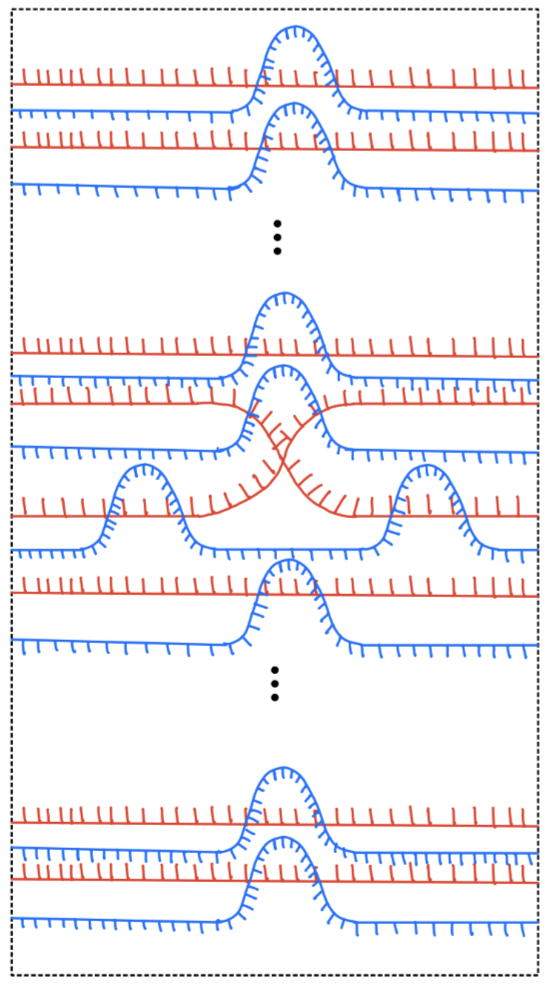
\includegraphics[scale = 0.55]{diagrams/local_systems_on_as_diagrams/1.png} 
    \caption{}
    \label{fig:your-label}
\end{figure}

we have the following associated quiver:

\begin{figure}[H] 
    \centering
    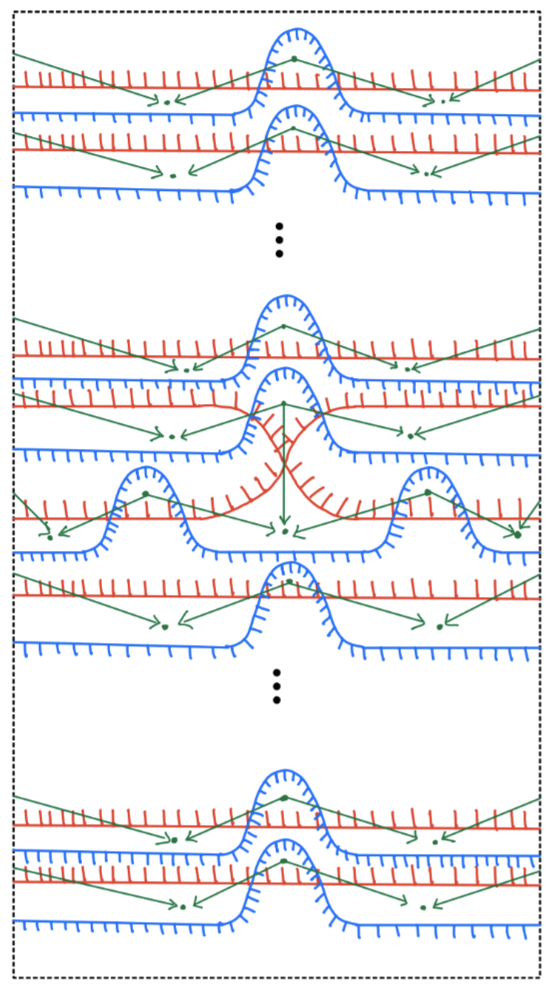
\includegraphics[scale = 0.55]{diagrams/local_systems_on_as_diagrams/2.png} 
    \caption{}
    \label{fig:your-label}
\end{figure}

Once we have an alternating strand diagram, we have the associated conjugate surface $L_{conj}$. Furthermore, we can embed the underlying undirected graph $\Gamma_{bi}$ of the quiver $Q$(i.e. the bipartite graph of the alternating coloring) in $L_{conj}$ in such a way that $L_{conj}$ deformation retracts to $\Gamma_{bi}$. Suppose we have a rank $1$ local system on the conjugate surface associated with $(M, \Lambda'_0, \Lambda'_\infty)$, then restricting to $Q$, we get a local system on $Q$. Note that the pullback, induced by the restriction map, between the space of local systems $H^1(L_{conj}, \C^*) \rightarrow  H^1(\Gamma_{bi},\C^*)$ is an isomorphism.

$H^1(\Gamma_{bi},\mathbb{C}^*)$ is isomorphic to $(\C^*)^{|Arr(Q)|}//(\C^*)^{|Vert(Q)|}$
here the group action is defined as the following : let $g_v \in (\C^*)^{|Vert(Q)|}$
(more precisely, $g_v := (g^{\delta_{w,v}})_{w \in Vert(Q)}$ where $\delta$ is the Kronecker delta),
then $g_v \cdot (x_a)_{a\in Arr(Q)}$ is 

\begin{itemize}
\item for entries with index $a$ such that the source of $a$ is $v$ i.e. $s(a) = v$, we have $g_v \cdot x_a$
\item for entries with index $a$ such that the target of $a$ is $v$ i.e. $t(a) = v$, we have $g_v^{-1} \cdot x_a$
\end{itemize}


Now we define the associated alternating sheaf on some regular cell complex refinement of the natural alternating strand diagram associated with a rank $1$ local systems on $Q$.

First, I will describe the special kind of regular cell complex associated with the alternating strand diagram called the regular cell complex refinement of the natural alternating strand diagram. I will define the refinement for each generator region and glue them to get the global regular cell complex.

\begin{definition}
Suppose we fix a generator region for the alternating strand diagram. Then we denote the $j^{th}$ crossing(numbering starts from left to right) the $i^{th}$ blue strand(numbering starts from top to bottom) crosses red strands as $c_{i,j}$. We will call the crossing between $i^{th}$ and $i+1^{th}$ red strand as $c$.
\begin{enumerate}[label = (\roman*)]
\item For each crossing $c_{i,j}$ we add 
\begin{itemize}
\item when $j$ is odd, locally near $c_{i,j}$ we have the following local diagram
\begin{figure}[H] 
    \centering
    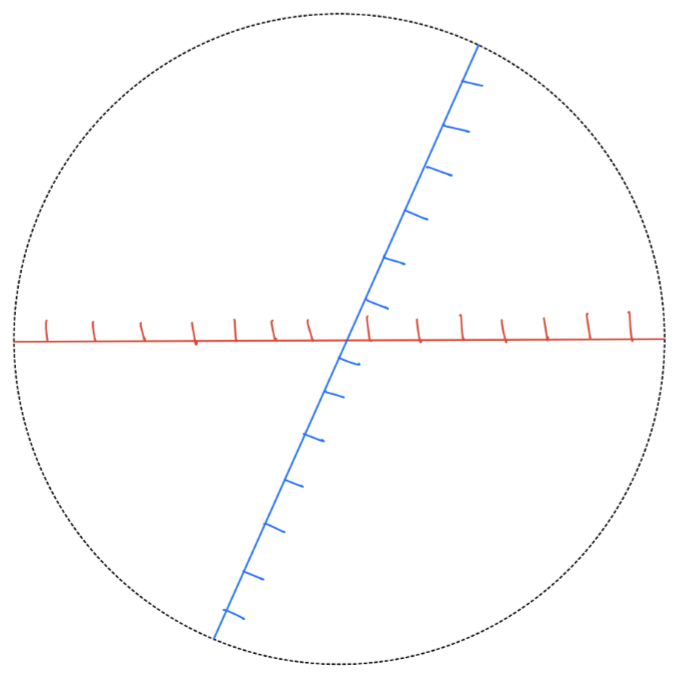
\includegraphics[scale = 0.55]{diagrams/local_systems_on_as_diagrams/3.png} 
    \caption{}
    \label{fig:your-label}
\end{figure}
then we add squiggly lines with co-orientations and end points to get
\begin{figure}[H] 
    \centering
    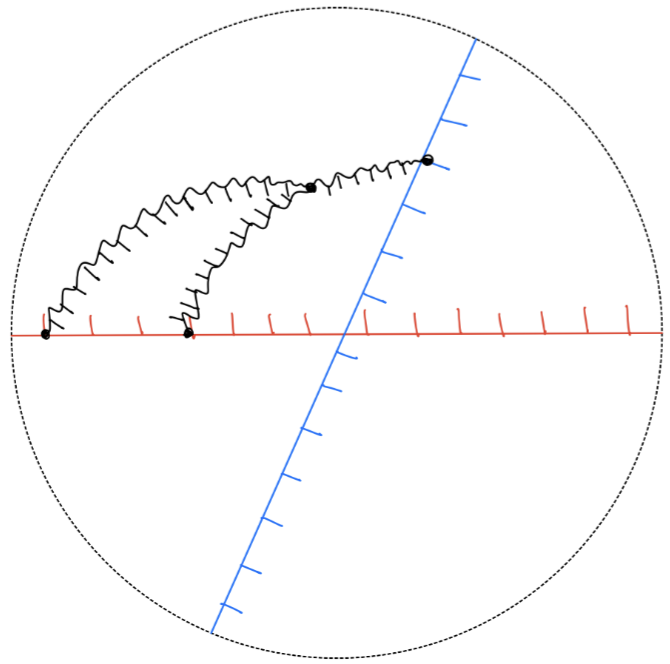
\includegraphics[scale = 0.55]{diagrams/local_systems_on_as_diagrams/4.png} 
    \caption{}
    \label{fig:your-label}
\end{figure}
We call the region marked with $*$ a crossing region.
\begin{figure}[H] 
    \centering
    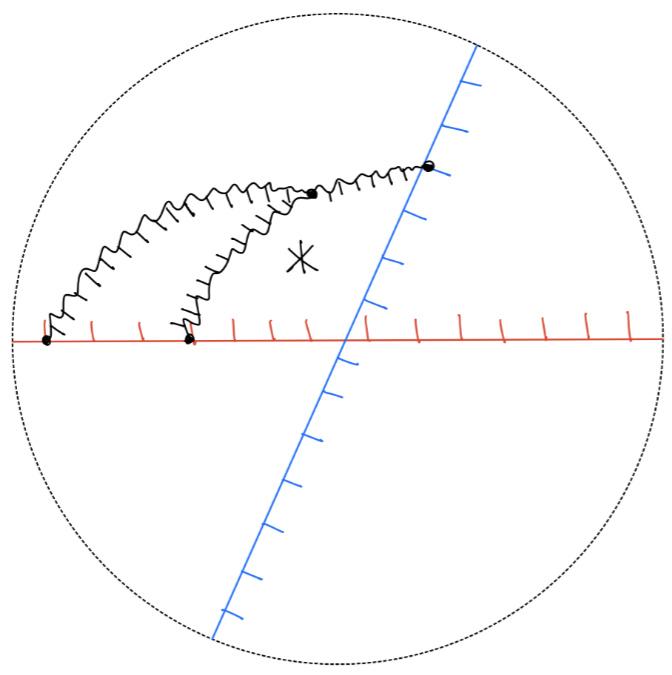
\includegraphics[scale = 0.55]{diagrams/local_systems_on_as_diagrams/5.png} 
    \caption{}
    \label{fig:your-label}
\end{figure}

\item when $j$ is even, locally near $c_{i,j}$ we have the following local diagram
\begin{figure}[H] 
    \centering
    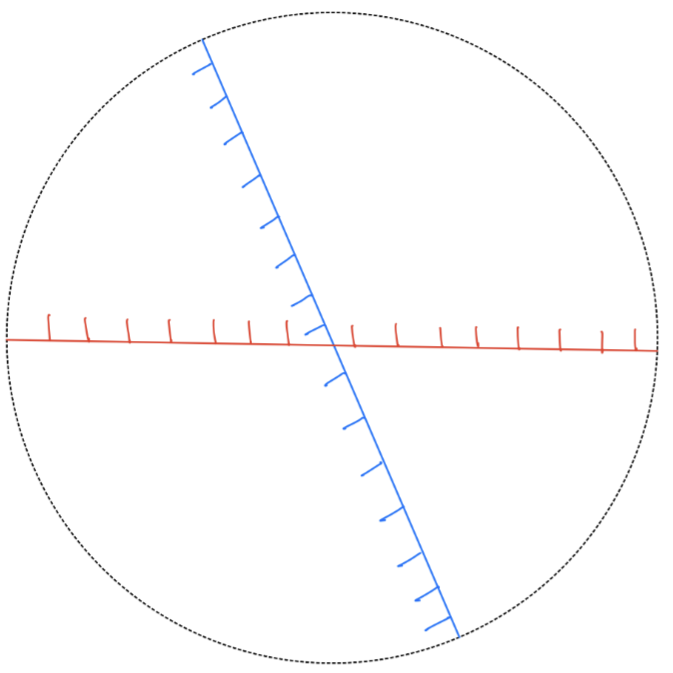
\includegraphics[scale = 0.55]{diagrams/local_systems_on_as_diagrams/6.png} 
    \caption{}
    \label{fig:your-label}
\end{figure}
then we add squiggly lines with co-orientations and end points to get
\begin{figure}[H] 
    \centering
    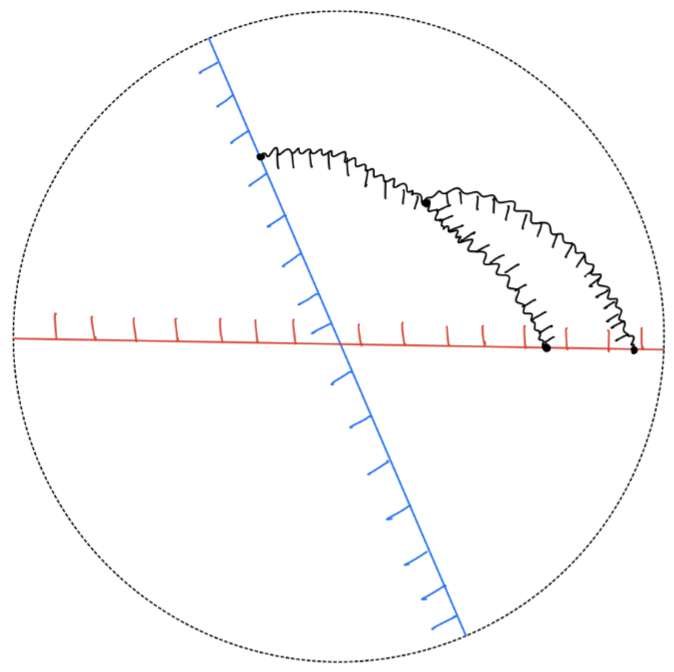
\includegraphics[scale = 0.55]{diagrams/local_systems_on_as_diagrams/7.png} 
    \caption{}
    \label{fig:your-label}
\end{figure}
We call the region marked with $*$ a crossing region.
\begin{figure}[H] 
    \centering
    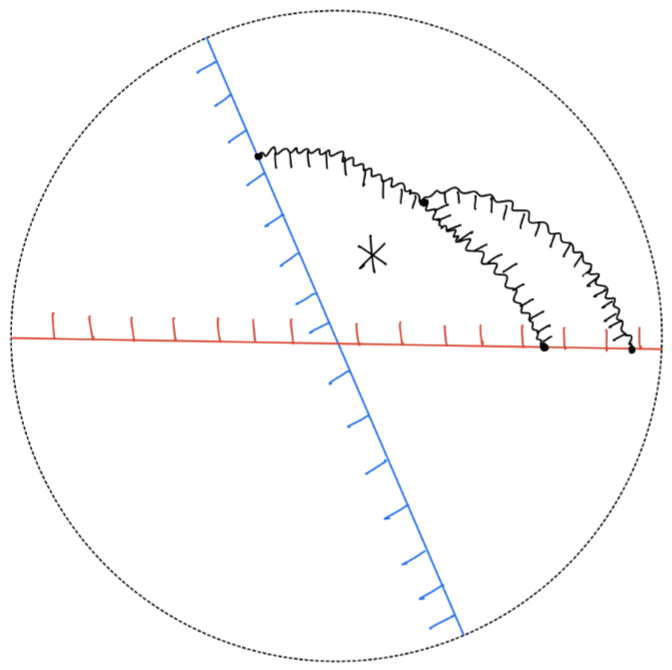
\includegraphics[scale = 0.55]{diagrams/local_systems_on_as_diagrams/8.png} 
    \caption{}
    \label{fig:your-label}
\end{figure}
\end{itemize}

\item For the crossing $c$, locally near the crossing, we have the following local diagram
\begin{figure}[H] 
    \centering
    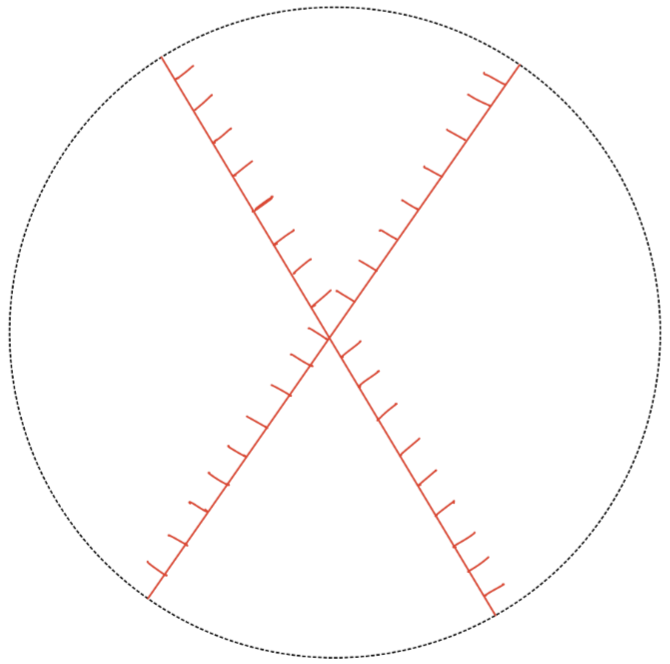
\includegraphics[scale = 0.55]{diagrams/local_systems_on_as_diagrams/9.png} 
    \caption{}
    \label{fig:your-label}
\end{figure}
then we add squiggly lines with co-orientations and end points to get
\begin{figure}[H] 
    \centering
    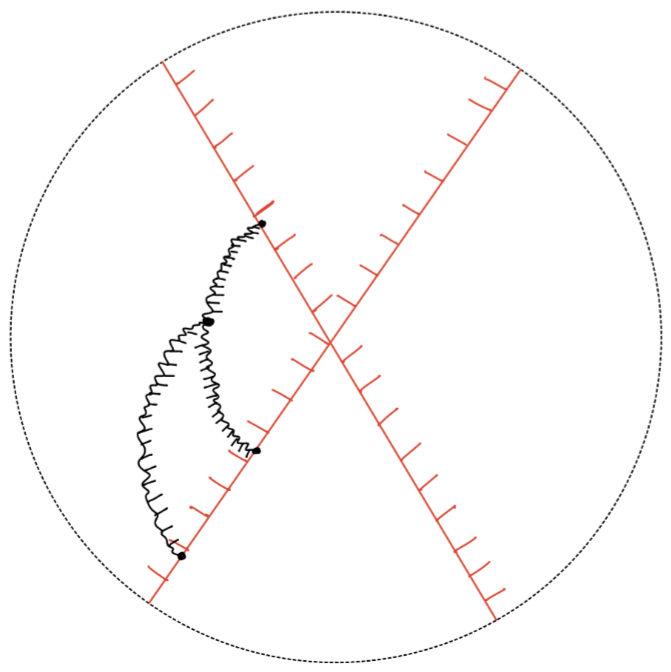
\includegraphics[scale = 0.55]{diagrams/local_systems_on_as_diagrams/10.png} 
    \caption{}
    \label{fig:your-label}
\end{figure}
We call the region marked with $*$ a crossing region.
\begin{figure}[H] 
    \centering
    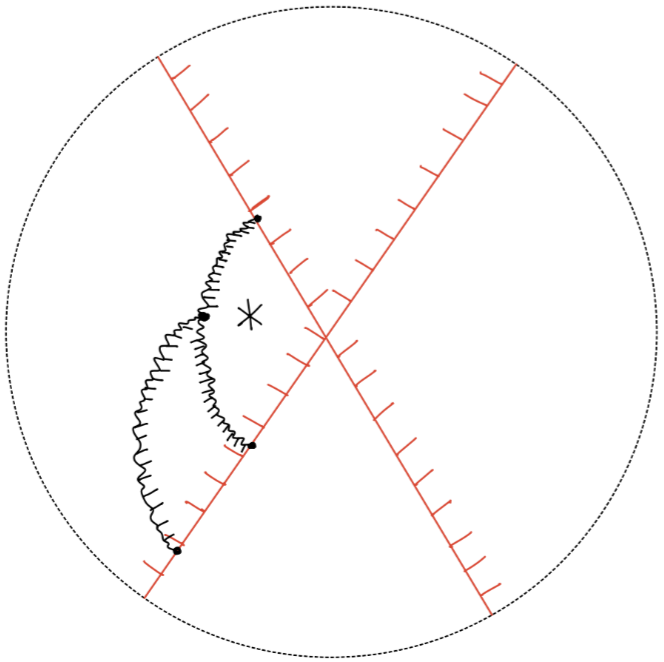
\includegraphics[scale = 0.55]{diagrams/local_systems_on_as_diagrams/11.png} 
    \caption{}
    \label{fig:your-label}
\end{figure}
\end{enumerate}

Below is the picture of a generator region of a natural alternating diagram:

\begin{figure}[H] 
    \centering
    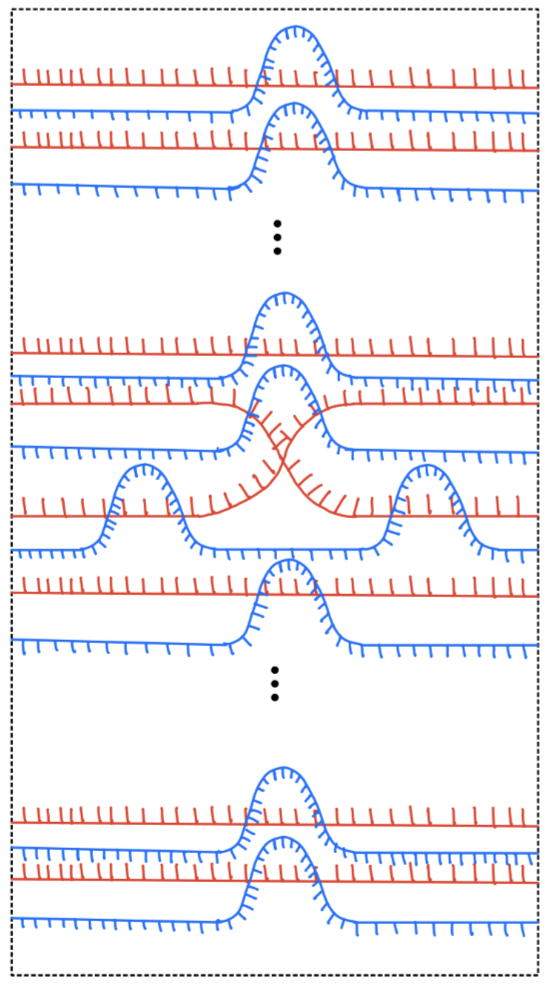
\includegraphics[scale = 0.55]{diagrams/local_systems_on_as_diagrams/12.png} 
    \caption{}
    \label{fig:your-label}
\end{figure}

and below is the picture of the regular cell complex refinement in a generator region:

\begin{figure}[H] 
    \centering
    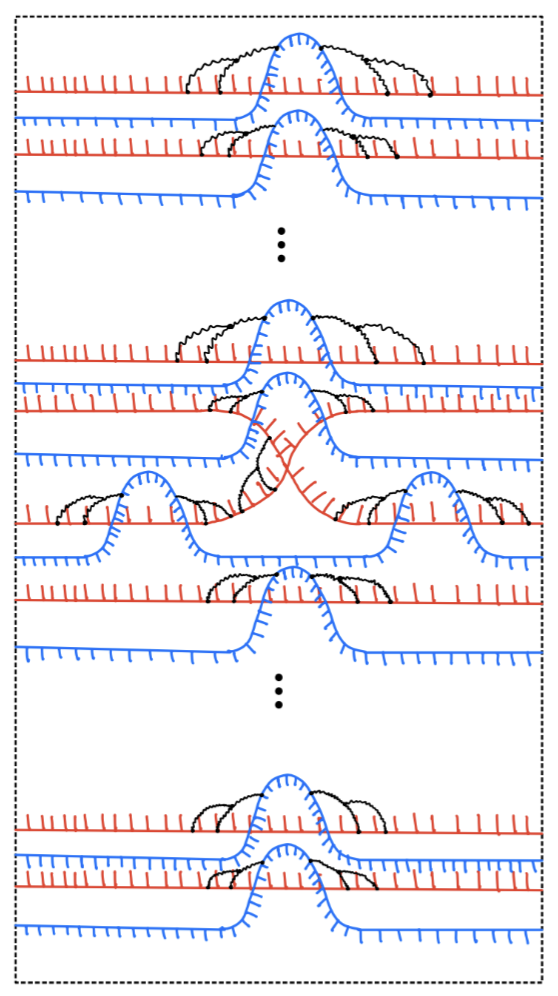
\includegraphics[scale = 0.55]{diagrams/local_systems_on_as_diagrams/13.png}
    \caption{}
    \label{fig:your-label}
\end{figure}
\end{definition}
Next, we fix an inter-generator region
\begin{figure}[H] 
    \centering
    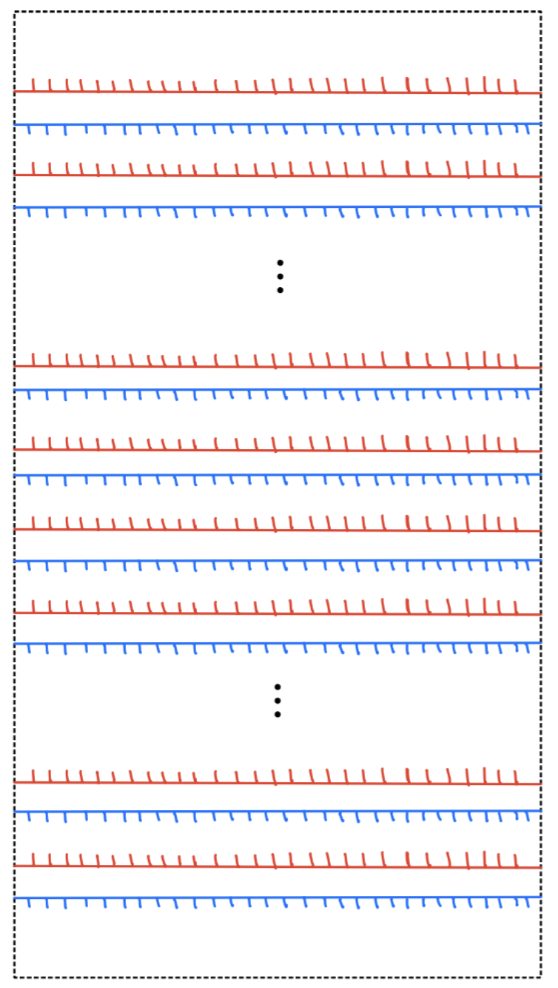
\includegraphics[scale = 0.55]{diagrams/local_systems_on_as_diagrams/14.png} 
    \caption{}
    \label{fig:your-label}
\end{figure}

add a vertical squiggly line co-oriented towards the left
\begin{figure}[H] 
    \centering
    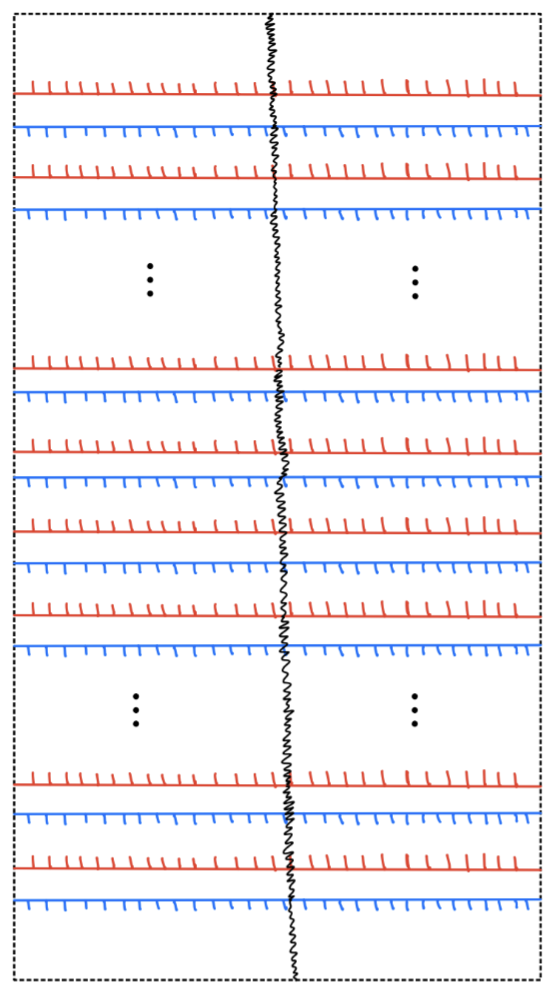
\includegraphics[scale = 0.55]{diagrams/local_systems_on_as_diagrams/15.png} 
    \caption{}
    \label{fig:your-label}
\end{figure}


Now I will describe a way to specify a constructible sheaf on the above regular cell complex refinement associated with the local system on $\Gamma_{bi}$. 

\begin{definition}
Suppose we have a local system on $Q$ which can be represented as an element $(x_A)_{a\in Arr(Q)}(\mathbb{C}^*)^{|Arr(Q)|}$:

\begin{enumerate}[label= (\roman*)]
\item stalk of the region where all the hairs are pointing outward is $\mathbb{C}[-1]$

\item stalk of the region where all the hairs(except the hairs on the squiggly lines) are pointing inward is $\mathbb{C}$

\item stalk of the crossing regions is $\mathbb{C}\xrightarrow{\times x_a}\mathbb{C}$ where $a$ is the arrow corresponding to the associated crossing.

\item rest of the stalks are $0$

\item the only nonzero genrization maps are from regions of type (\Rn{3}) to (\Rn{1}), from (\Rn{1}) to (\Rn{2}), or from (\Rn{2}) to (\Rn{2})(the ones corresponding to vertical squiggly lines in the inter-generator regions)
\end{enumerate}

The maps from (\Rn{3}) to (\Rn{1}) are
\[
  \begin{tikzcd}
    \mathbb{C} \arrow{r}{\times 1} & \mathbb{C} \\
    \mathbb{C}\arrow{u}{} \arrow{r}{}& 0\arrow{u}{}
  \end{tikzcd}
\]

The maps from (\Rn{1}) to (\Rn{2}) are
\[
  \begin{tikzcd}
	0 \arrow{r}{} & \mathbb{C} \\
    \mathbb{C}\arrow{u}{} \arrow{r}{\times 1}& \mathbb{C}\arrow{u}{}
  \end{tikzcd}
\]

The maps from (\Rn{2}) to (\Rn{2}) are identity maps.
\end{definition}

Note that the group action maps a constructible sheaf to the isomorphic constructible sheaf. Therefore, we have a well-defined map
$H^1(L_{conj},\mathbb{C}^*)\rightarrow \mathcal{M}_1(M,\Lambda',\{\sigma_{z\ll 0},\sigma_{z\gg 0}\};\C)$ where $\Lambda' = \Lambda'_0 \coprod \Lambda'_\infty$, $\sigma_{z\ll 0}$ is a point in the region containing $0$, and $z\gg 0$ is a point in the region containing $\infty$.
\pagebreak